\chapter{The LHC accelerator and the CMS experiment}\label{chapter:lhc-cms}
\section{The Large Hadron Collider}\label{sec:lhc}

The Large Hadron Collider (LHC) at the European Organisation for Nuclear Research (CERN)~\cite{Bruning:782076}, in Geneva, Switzerland is the highest-energy particle accelerator constructed to date. 
%It is designed to operate at a centre-of-mass energy of 14\TeV, through two 7\TeV proton beams travelling in 2808 bunches, with each bunch containing up to $1.15 \times 10^{11}$ protons, at a collision rate of 25\ns, which corresponds to a design instantaneous luminosity of $10^{34}\percms$~\cite{Bayatian:2006zz}. 
It is designed to operate at a centre-of-mass energy of 14\TeV at a design instantaneous luminosity of $10^{34}\percms$~\cite{Bayatian:2006zz}. 
The LHC is also capable of accelerating heavy-ions, which is usually done for one month a year with lead ions with up to 2.76\TeV per nucleon being used for lead-lead or lead-proton collisions.

The beams collide at four interaction points around the LHC, with one of the four major experiments being based at each of them. 
The experiments are: A Toroidal LHC Apparatus (ATLAS)~\cite{Aad:2008zzm} and the Compact Muon Solenoid (CMS)~\cite{oldcms} detectors, which are the two multi-purpose experiments; the Large Hadron Collider beauty (LHCb) experiment~\cite{Alves:2008zz}, which specialises in b-physics and A Large Ion Collider Experiment (ALICE)~\cite{Aamodt:2008zz}, which, as the name suggests, specialises in heavy ion physics.
Three smaller experiments are situated close to one of the four main experiments and use the same collision points.
Both the TOTal Elastic and diffractive cross section Measurement (TOTEM)~\cite{Anelli:2008zza} and LHC-forward (LHCf)~\cite{Adriani:2008zz} experiments study diffractive physics in the very-forward regions of collisions at the CMS and ATLAS experiments' collision points, respectively.
Monopole and Exotics Detector At the LHC (MoEDAL)~\cite{Pinfold:2009oia} shares the LHCb experiment's cavern and performs direct searches for magnetic monopoles and highly ionising stable and pseudo-stable massive particles.

Currently there are three planned phases of operation for the LHC: ``Phase-0'' will see the preparations for 14\TeV operations; ``Phase-I'' will see the accelerator prepared for high luminosity operations; and ``Phase-II'' will see modifications for very high luminosity operations~\cite{ECFA}. 
Figure~\ref{fig:lhc-planning} illustrates the timescales of the current plans for the operation and shutdown periods of the LHC.
Any proposed upgrades of the detectors will naturally have to coincide with the shutdowns of the LHC.

\begin{figure}[htb]
\begin{center}
\vspace*{5mm}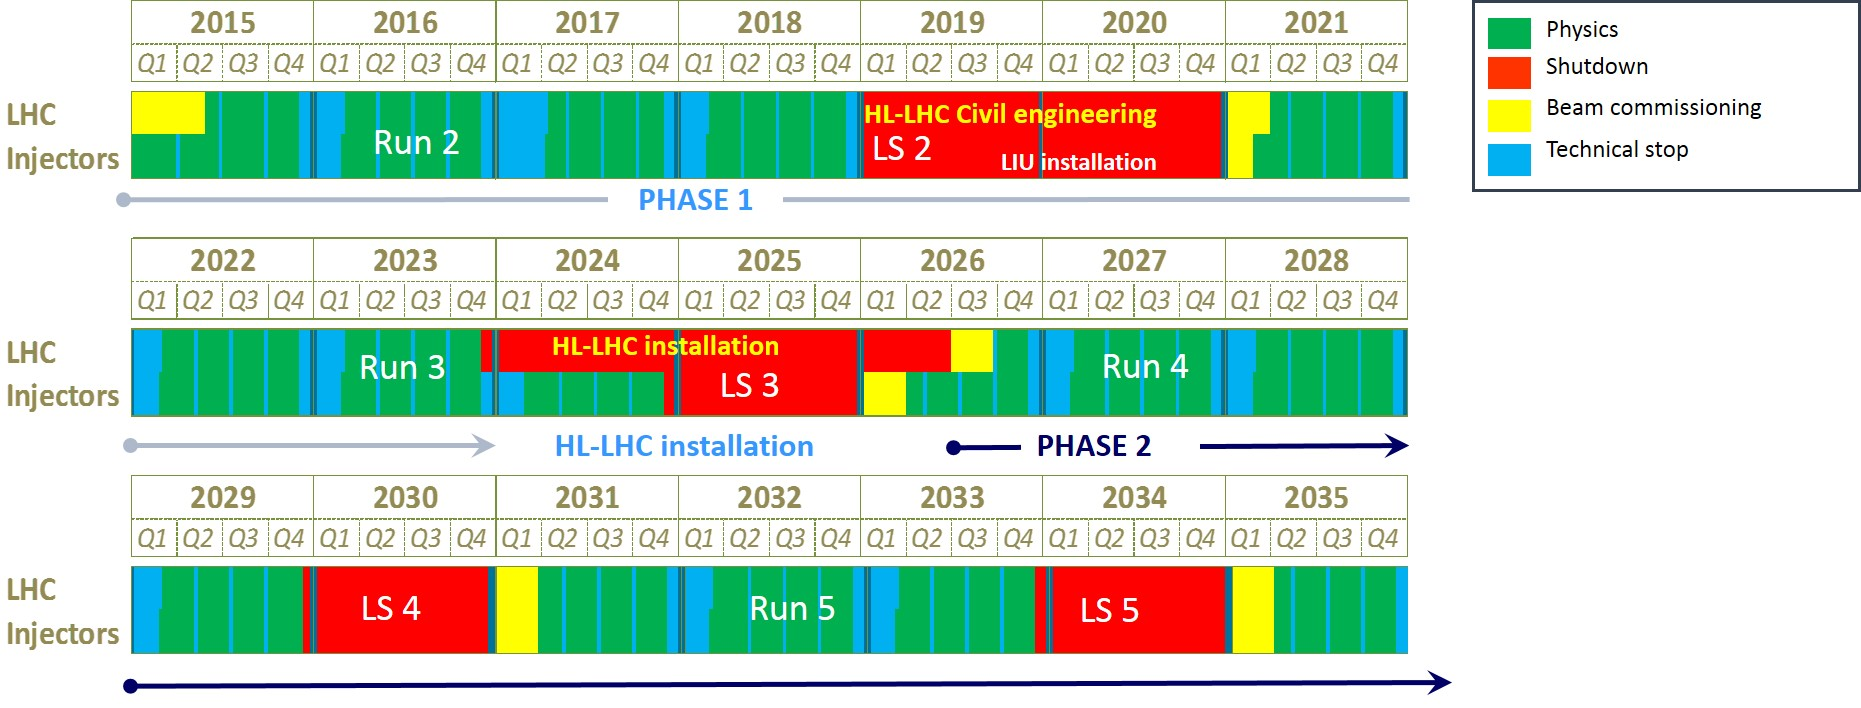
\includegraphics[width=0.99\textwidth]{figs/lhc/LHC-Planning.jpg}
\caption{Overview of the plan for the LHC and its injectors from 2015 to 2035~\cite{P2TrackerTDR}. Data taking for physics is indicated in green, long shutdowns in red, beam commissioning in yellow and technical stops in blue.}
\label{fig:lhc-planning}
\end{center}
\end{figure}

\subsection{Accelerator Complex}\label{subsec:acceleratorComplex}
When operating in proton-proton mode, the preparation of the LHC beams starts at Linear accelerator 2 (Linac2). 
Protons from a hydrogen gas source are accelerated to 50\MeV and are injected into the Proton Synchrotron Booster (PSB) which accelerates the protons to 1.4\GeV before injection into the Proton Synchrotron (PS). 
In the PS, the protons are accelerated to 26\GeV and are injected into the Super Proton Synchrotron (SPS) where they are accelerated to 450\GeV before finally entering the LHC, as illustrated in Figure~\ref{fig:cern-accelerator-complex}. 
%% No necessary - no considering HI collision
%When operating with lead ions, Linear accelerator 3 (Linac3) is used to initially accelerate the ions before injecting them into the Proton Synchrotron Booster, before the ions use the same accelerators as the protons do to prepare them for use in the LHC~\cite{Bruning:782076}. 

\begin{figure}[htb]
\begin{center}
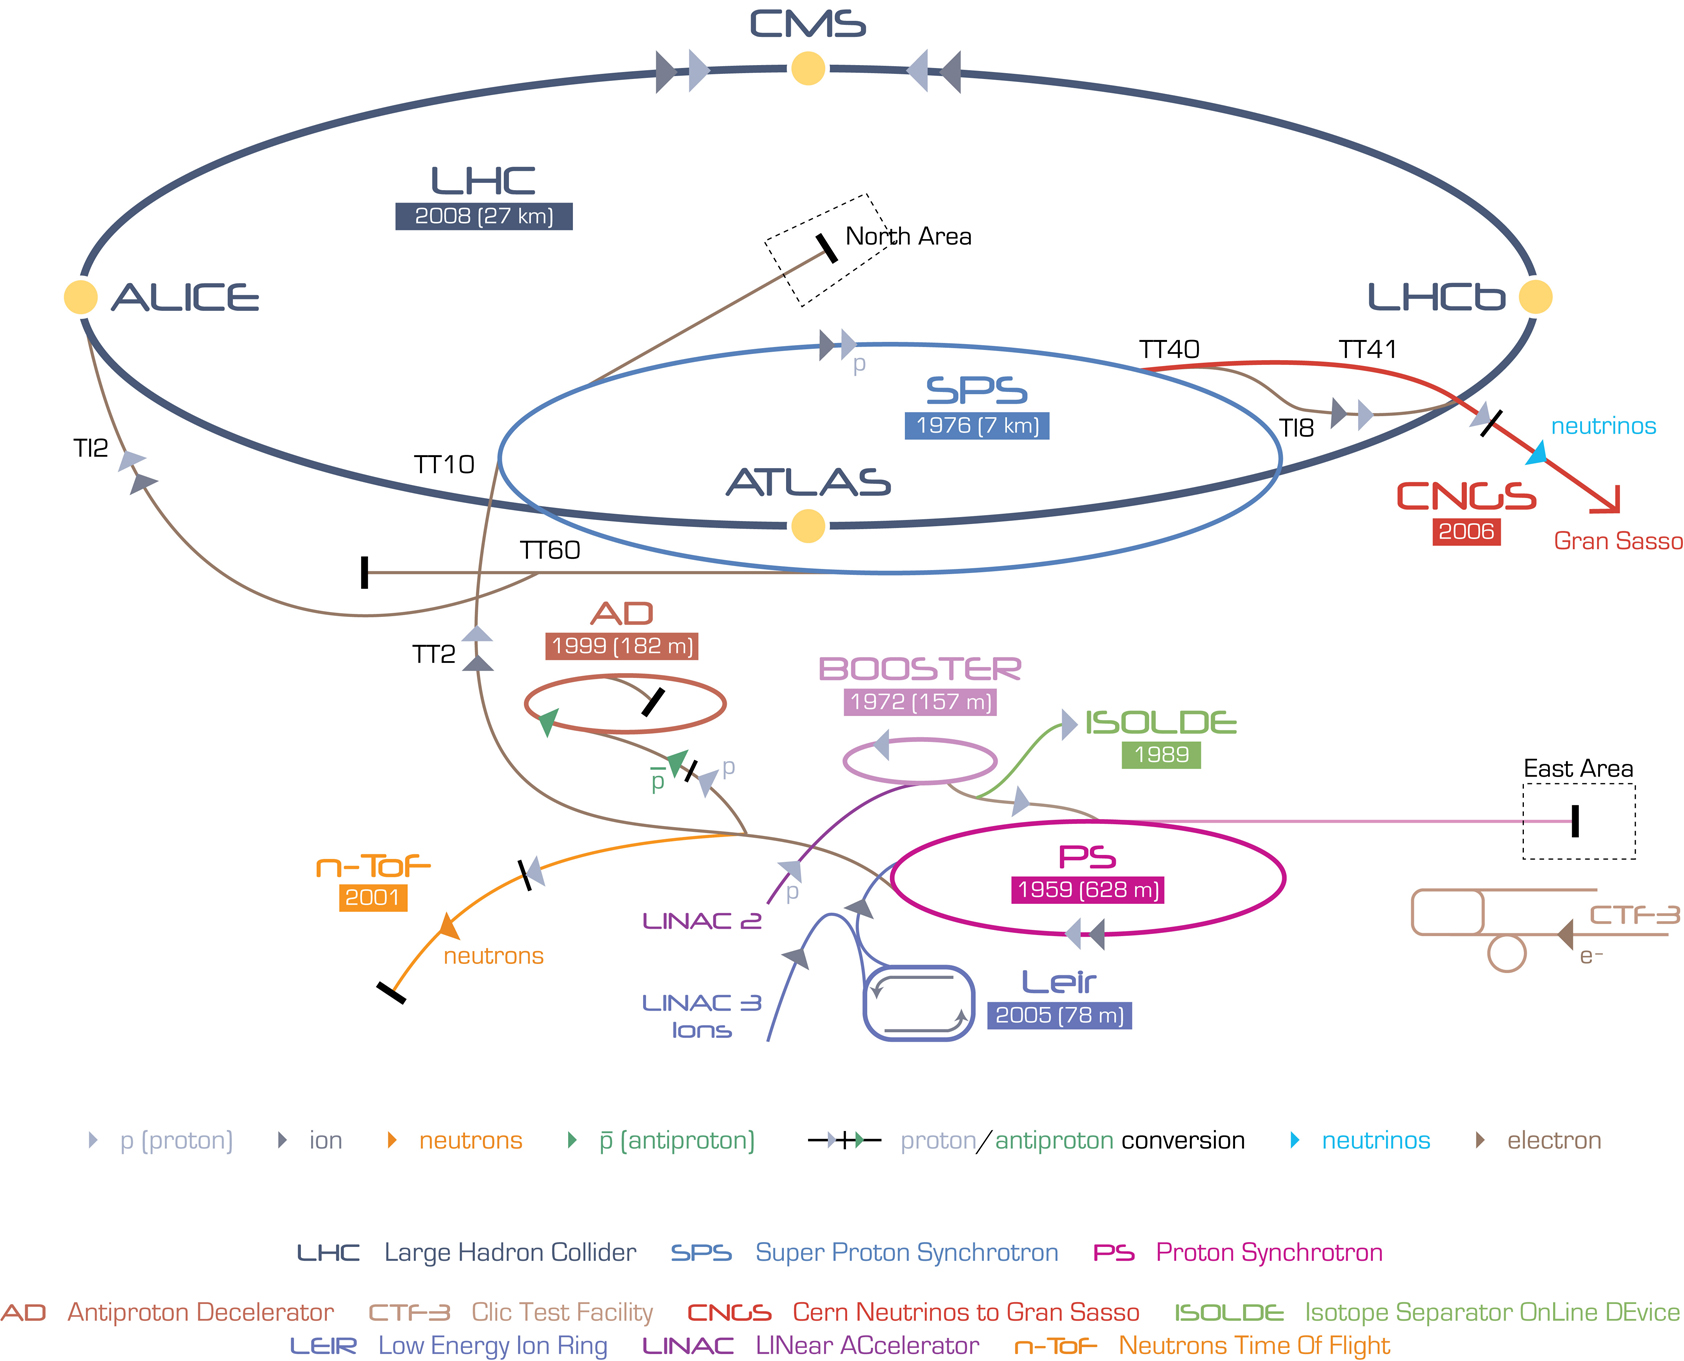
\includegraphics[width=0.97\textwidth]{figs/lhc/Cern-Accelerator-Complex.jpg}
\caption{CERN complex, including the various linear accelerators, synchrotrons, LHC, LHC detectors and other aspects of the complex~\cite{Marcastel:1621583}.}
\label{fig:cern-accelerator-complex}
\end{center}
\end{figure}

Sixteen Radio Frequency (RF) cavities (eight per beam), each operating at frequency of 400\MHz, delivering a maximum of 2 MV at an operational temperature of 4.5K, are used to accelerate the two beams up to their designed operational energies of 7\TeV over the course of about twenty minutes.
Each of the two beams are accelerated in separate beam pipes, circulating in opposite directions.
The beams requires 1232 dipole magnets to bend them along their circular path and 392 quadrupole magnets to focus them, with each magnet producing a 8.3T field whilst operating at 1.9K.
A more detailed description of the LHC accelerator chain at CERN can be found in~\cite{Schindl:397574}. 

\subsection{Motivation}\label{subsec:lhcMotivation}
The core motivations behind the LHC are to shed light on the nature of the electroweak symmetry breaking, for which the Higgs was presumed and found to be responsible, and to probe the consistency of the SM above the \TeV level through precision measurements of SM parameters and the Higgs mechanism.
Extensions of the SM, such as SUSY theories, additional dimensions or new fundamental forces and particles are expected to emerge at and above the \TeV level, giving the potential to ascertain whether these theories have any basis beyond mere conjecture~\cite{Bayatian:2006zz}.
%In order to explore and permit the discovery of physics above the \TeV level, the total centre of mass energy has to be greater than the energy region being explored as, due to the composite nature of the proton, only a fraction of the collision centre-of-mass energy is available.
%Access to physics beyond the \TeV level is not excluded	however, as some signals would be ``unmissable'', but the majority of physics would be limited by statistics.
As shown in Figure~\ref{fig:crossSections}, the production cross section of the Higgs boson and hypothesised SUSY particles, if they have \TeV masses (and exist), are predicted to be many orders of magnitude smaller than both their associated backgrounds and the total inelastic cross section.

\begin{figure}[htb]
\begin{center}
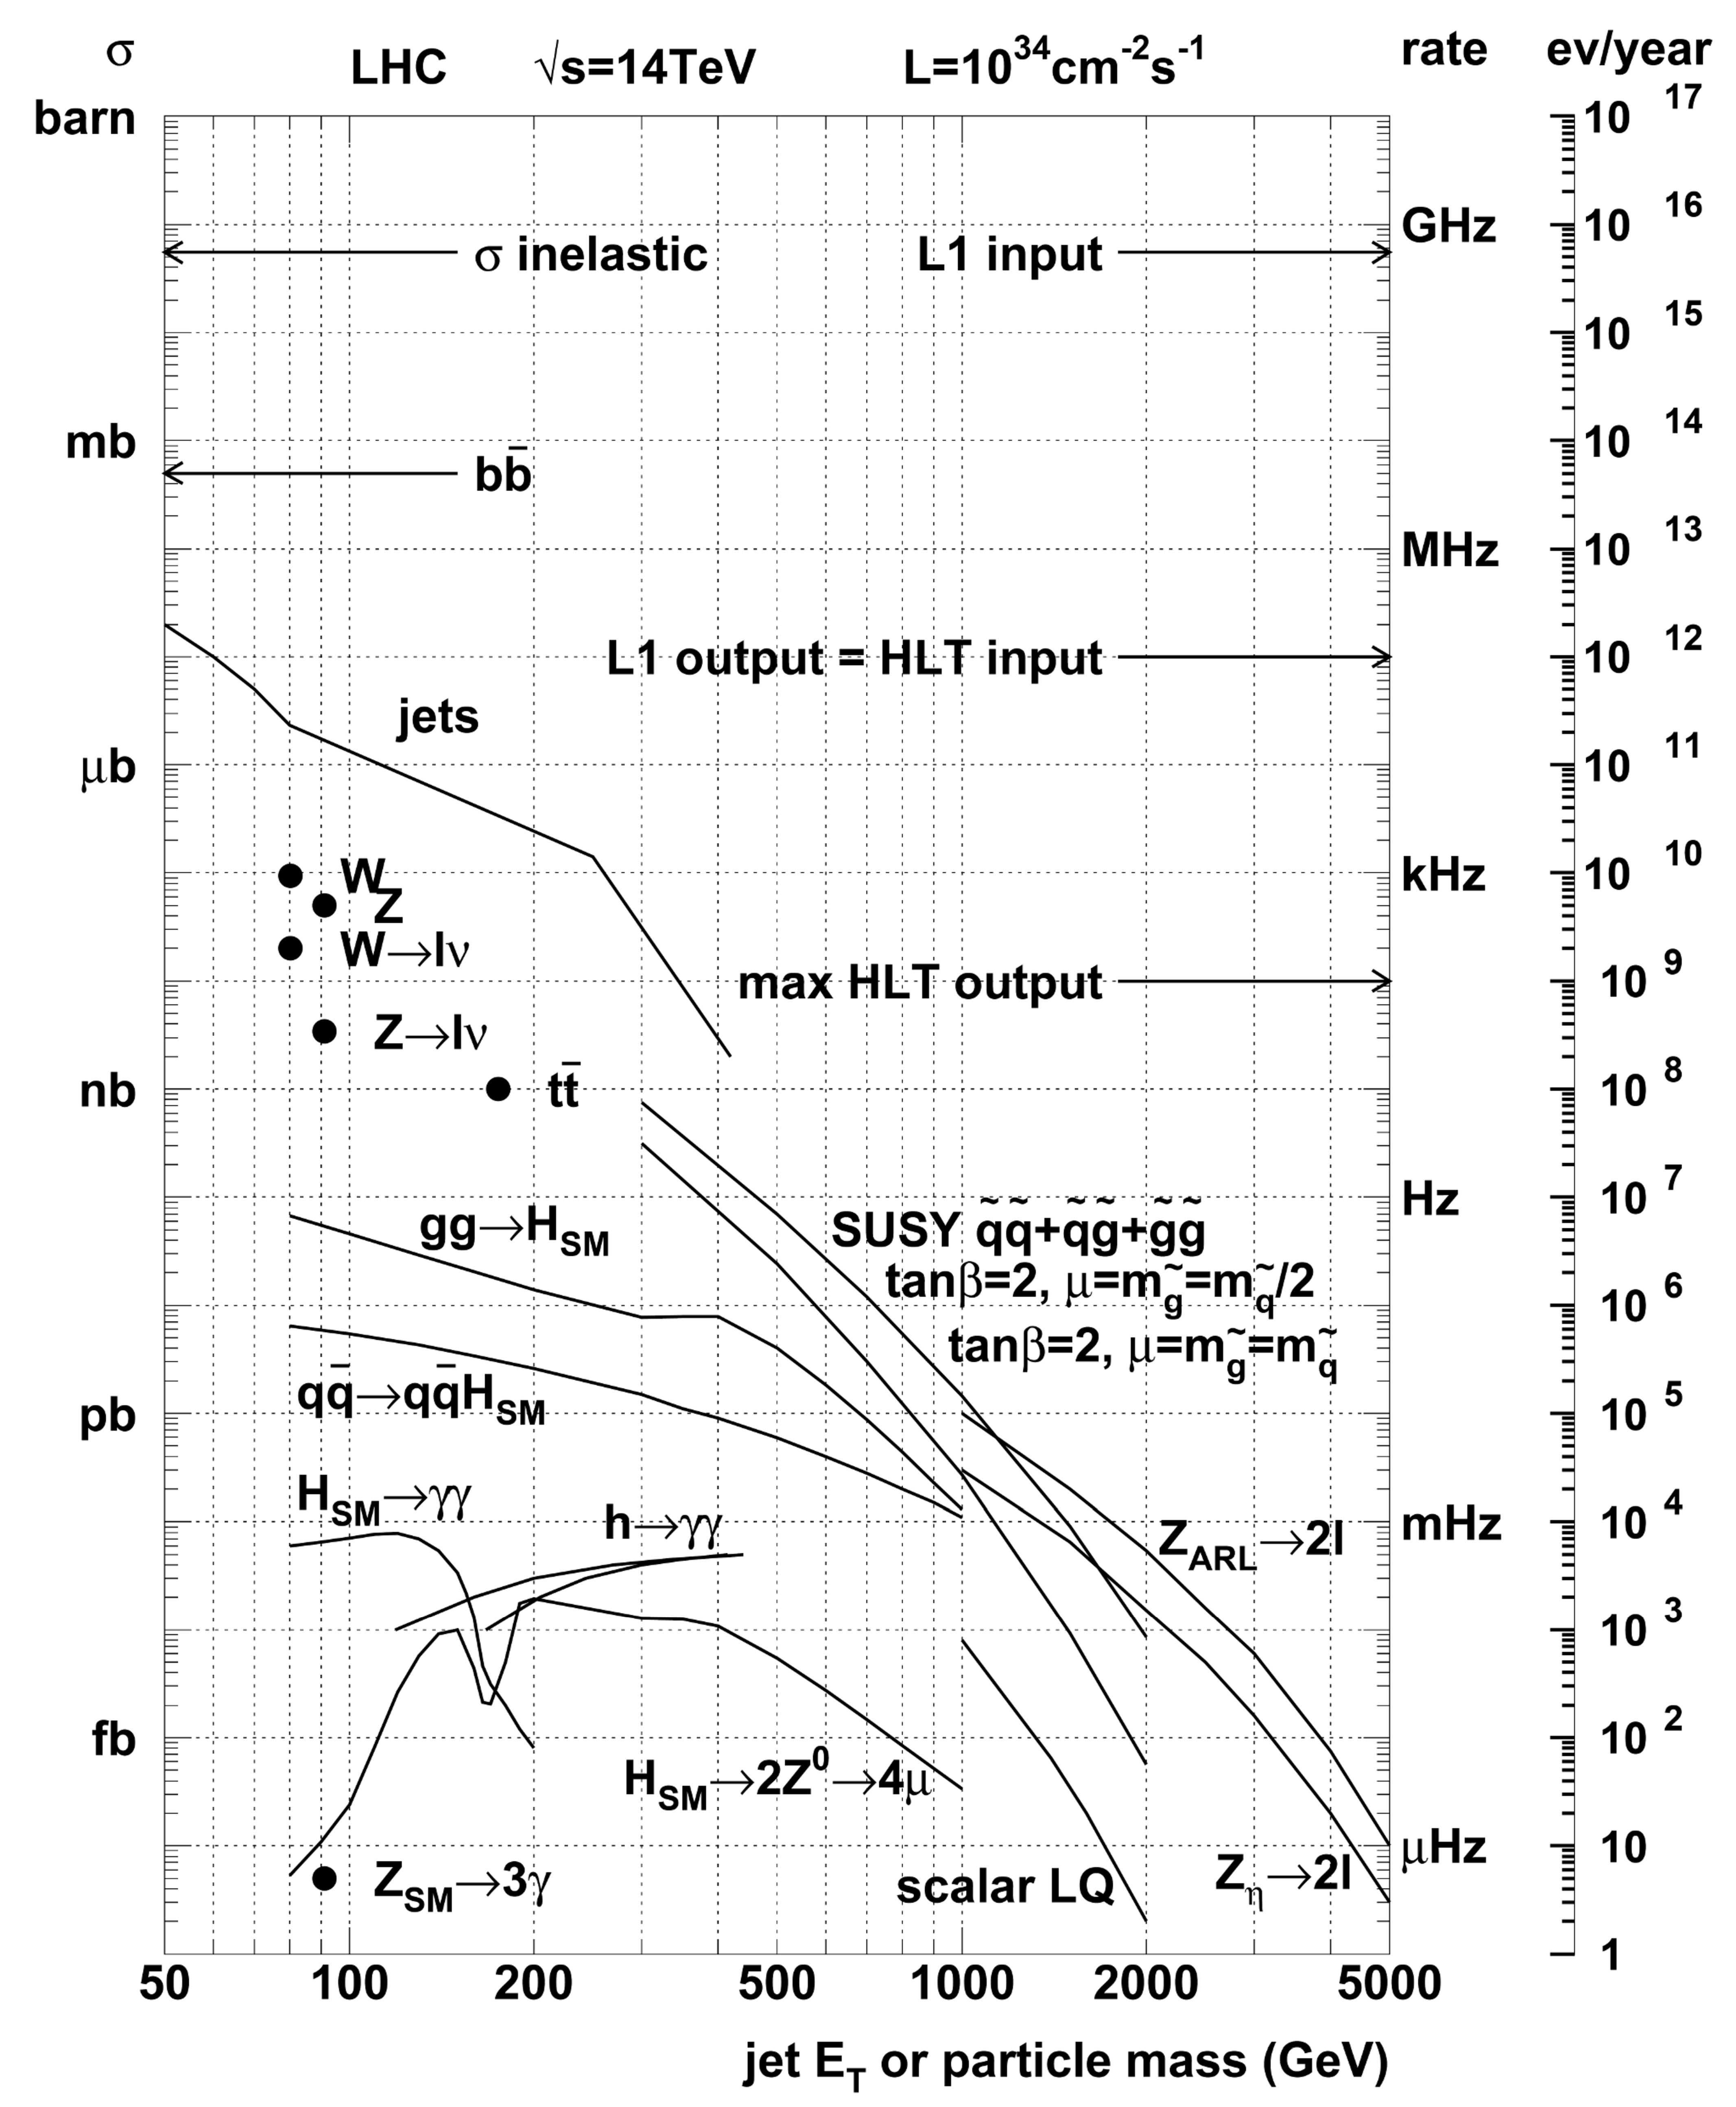
\includegraphics[width=0.70\textwidth]{figs/cms/crossSections.pdf}
\caption{The inclusive proton-proton cross sections at $\sqrt{s} = 14\TeV$ and the production frequency for various physics processes, as a function of jet \ET or mass, expected at the LHC at a luminosity of $10^{34}\percms$~\cite{Dasu:2000ge}.}
\label{fig:crossSections}
\end{center}
\end{figure}

Consequently, in order to perform measurements of such processes, as well as precision measurements of SM parameters, the LHC was designed to be capable of achieving an instantaneous beam luminosity of up to $10^{34}\percms$.
Such a high instantaneous luminosity was achieved by delivering protons in 2808 bunches per beam, with each bunch containing up to $1.15 \times 10^{11}$ protons, which at design luminosity will separated by 25ns to provide a bunch collision rate of up to 40\MHz.
The instantaneous luminosity is further increased by squeezing the proton bunches to enhance the number of simultaneous inelastic proton-proton interactions during each bunch crossing.
These multiple simultaneous collisions are named pile-up (\PU) interactions and usually consist of soft QCD interactions~\cite{Bruning:782076,Ball:2007zza}.
\PU can occur both within and adjacent to an event's bunch crossing, known as \emph{in-time} and \emph{out-of-time} \PU respectively.
%An average \PU of 

This high event rate presents the experiments' data acquisition and readout challenges, whilst retaining excellent signal-to-background resolution and sufficient radiation hardness in order to withstand the expected fluence.
%% No need to mention HI mode
%The primary motivation behind operating the LHC in a heavy-ion mode is to search for evidence of the plasma of quarks and gluons, which is made possible through the resultant production of QCD matter under extreme temperature, density and low momentum fractions of partons~\cite{Baur:687318}.

\section{The Compact Muon Solenoid}\label{sec:cms}
\subsection{Overview}
The Compact Muon Solenoid (CMS)~\cite{oldcms} is a large, general purpose, hermetic particle detector and the smaller of the two multi-purpose experiments operating at the LHC.
Figure~\ref{fig:cms-cutaway} illustrates how the experiment and its sub-detectors are divided into a central cylindrical barrel section and two endcap disk sections at each end of the barrel.
A superconducting solenoid encompasses, moving from the interaction point at the centre of the detector outwards, an all-silicon tracking detector, a homogeneous lead tungstate ($PbWO_{4}$) electromagnetic calorimeter (ECAL) and a hadronic calorimeter (HCAL) comprised of plastic scintillating tiles interspaced with brass absorbers.
Beyond the solenoid there is an outer hadronic calorimeter (HO) and interspaced between the iron return yoke are three different types of Muon Detectors.
There is also a pair of very-forward calorimeters (HF) to further extend the hadronic calorimetry coverage to ensure good dijet mass and \MET resolutions.

\begin{figure}[htb]
\begin{center}
\includegraphics[width=\textwidth]{figs/cms/cms_160312_02.pdf}
\caption{Cutaway diagram of CMS’s layers, illustrating its onion-like nature and the location of the detecting technologies within~\cite{Sakuma:2013jqa}.}
\label{fig:cms-cutaway}
\end{center}
\end{figure}

These detectors were designed to investigate the wide range of physics phenomena in the LHC's physics program, resulting in the accurate and precise identification and measurement of electrons, photons, jets and muons over both a large energy and momenta range.
%% Explained above
%Sufficient radiation hardness for the expected high fluence and data acquisition and trigger systems required to handle to event rate of the LHC environment had to be considered in the design of the various detectors.

The coordinate system adopted by the CMS experiment has its origin at the nominal interaction point at the centre of the detector. 
The z-axis is parallel to the anti-clockwise proton beam, the x-axis points towards the centre of the LHC, and the y-axis points vertically upwards.
The azimuthal angle, $\phi$, is the angle measured from the x-axis in the x-y plane and the polar angle, $\theta$, is the angle measured clockwise relative to the positive z-axis.
Pseudorapidity, defined as $\eta \equiv -ln\tan(\theta/2)$, is usually used in lieu of $\theta$, as $\eta$ is Lorentz invariant along the z-axis and is approximately equivalent to rapidity, $y \equiv \frac{1}{2} ln(E+p_{z}/E-p_{Z})$, for highly relativistic particles. 

\subsection{Tracker}\label{subsec:tracker}
The tracker, measuring 5.8m with a 2.5m radius over a pseudorapidity range of $|\eta| < 2.5$, surrounds the interaction point.
The tracker is designed to provide precision trajectory measurements of charged particles emerging from collisions and precise reconstruction of vertices at high efficiencies, whilst operating in a harsh radiation environment (maximum flux $\approx 10^{7}/s$) and minimising the number charged particles interacting with the tracker.

\begin{figure}[htb]
\begin{center}
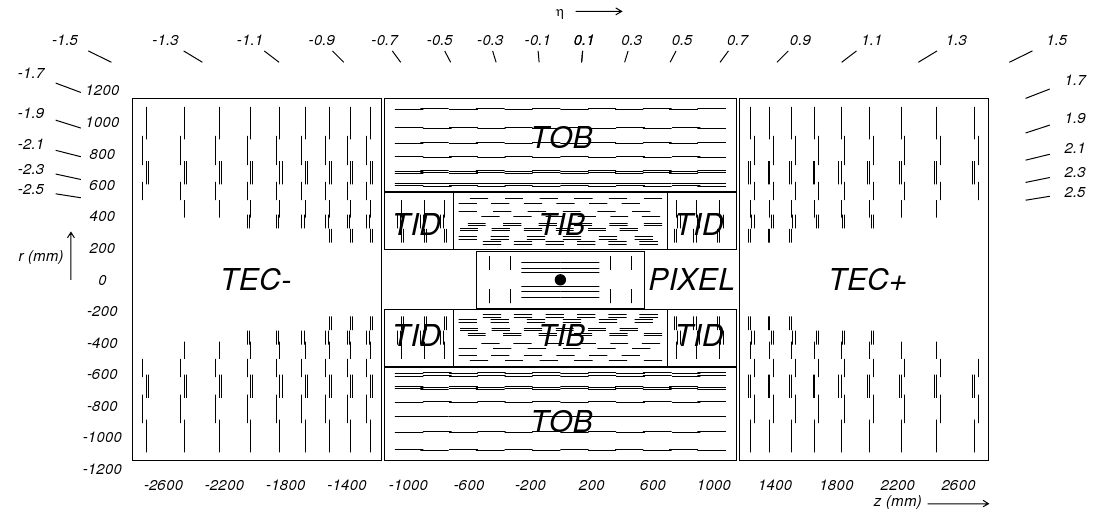
\includegraphics[width=0.97\textwidth]{figs/cms/fig_cmstracker.png}
\caption{Schematic of the CMS tracking detector, displaying the interaction point in the centre and the location of the sub-detectors and, through the arrangement of the lines, their modules. The double lines present in the microstrip tracker denote modules with double-sided sensors~\cite{Sprenger:2010ss}.}
\label{fig:tracker}
\end{center}
\end{figure}

Silicon fulfils these requirements and is used in both the inner pixel and microstrip detectors.
Figure~\ref{fig:tracker} illustrates how the various parts of the silicon microstrip detector surround the inner pixel detector.
The high particle multiplicity expected closest to the interaction point requires high granularity pixels provide in order to ensure a low channel occupancy ($< 1\%$).
For radii above 20\cm however, the particle flux is sufficiently low enough that microstrips can be used without compromising track reconstruction efficiency.
The low occupancy of the tracker results in a tracking efficiency of greater than 99\% for charged particles with $\pT > 1 \GeV$.
In the presence of the solenoid's magnetic field, the tracking system has an impact parameter resolution of approximately $10\mum$ and momentum resolutions between $1.5\%$ and $3.0\%$ for charged particles with $\pT = 100\GeV$ and $1 < \pT < 100\GeV$ respectively~\cite{Khachatryan:2010pw,Chatrchyan:2014fea}.

%In the presence of the solenoid's magnetic field, the tracking system has an impact parameter resolution of approximately $10\mum$ for charged particles with $\pT = 100\GeV$ and momentum resolutions between $1.5\%$ and $3.0\%$ for charged particles with $1 < \pT < 100\GeV$~\cite{Khachatryan:2010pw,Chatrchyan:2014fea}.

% Tracker performance plots
%\begin{figure}[htb]
%\begin{center}
%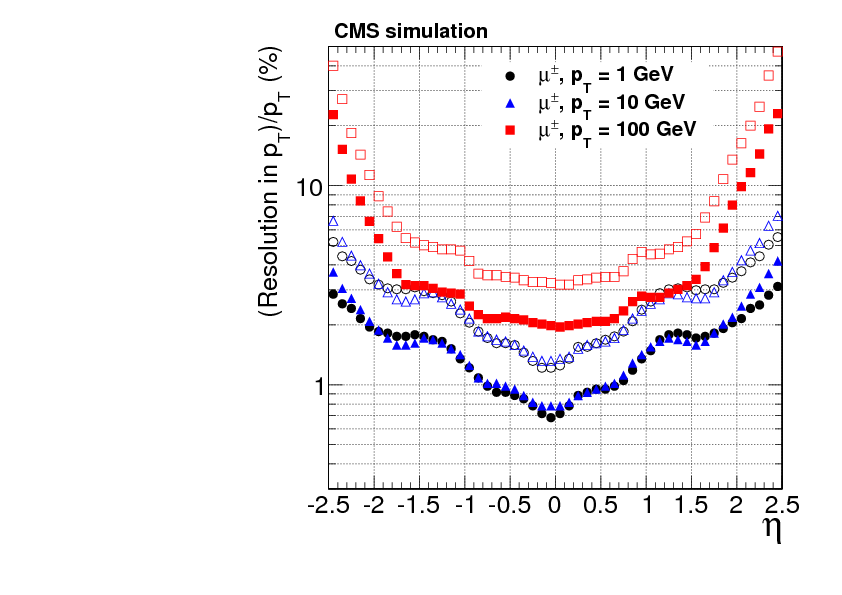
\includegraphics[width=0.47\textwidth]{figs/cms/figs_2011_trackPerformance_MC_SingleParticles_mu_resolutionPtVsEta.png}
%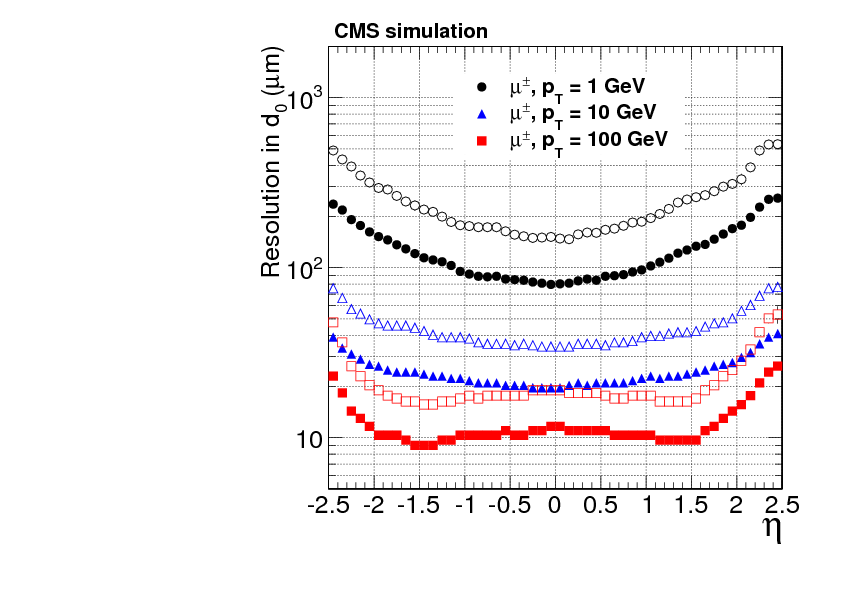
\includegraphics[width=0.47\textwidth]{figs/cms/figs_2011_trackPerformance_MC_SingleParticles_mu_resolutionD0VsEta.png}
%\caption{The relative \pT and  ptdown 1~\cite{Chatrchyan:2014fea}.}
%\label{fig:pixel}
%\end{center}
%\end{figure}

% figs/cms/trackerResolution_sumpt_x.pdf and trackerResolution_sumpt_z.pdf
%Brondolin:2016pxw and https://twiki.cern.ch/twiki/bin/view/CMSPublic/TrackingPOGPlotsICHEP2016

\subsubsection{Silicon Pixel Tracker}
The original silicon pixel detector for the CMS experiment was comprised of three 53.3$\cm$-long barrel layers at mean radii of 4.4\cm, 7.3\cm and 10.2\cm respectively, and two endcap disks either side of the barrel at $|z| = 34.5$ and 46.5\cm respectively, that extend from $r = 6.0$ to 15\cm.
Figure~\ref{fig:pixel} shows an installed pixel detector endcap disk and a half disk being reinstalled around the LHC beam pipe before the start of Run 2 operations.
The pixel sensors consist of n$^{+}$-type implants on n-type silicon which are connected by indium bump-bonds to highly integrated ReadOut Chips (ROCs).
Each of the 66 million pixels measures $100 \times 150\mum^{2}$, covering a total surface area of 1.06 m$^{2}$, resolutions of 10\mum in $r-\phi$ and 20\mum in $z$, providing the granularity required to have a high track reconstruction efficiency and to be able to precisely calculate the track impact parameters and vertex position.

%CMS pixel picture
\begin{figure}[htbp]
\begin{center}
\vspace*{2mm}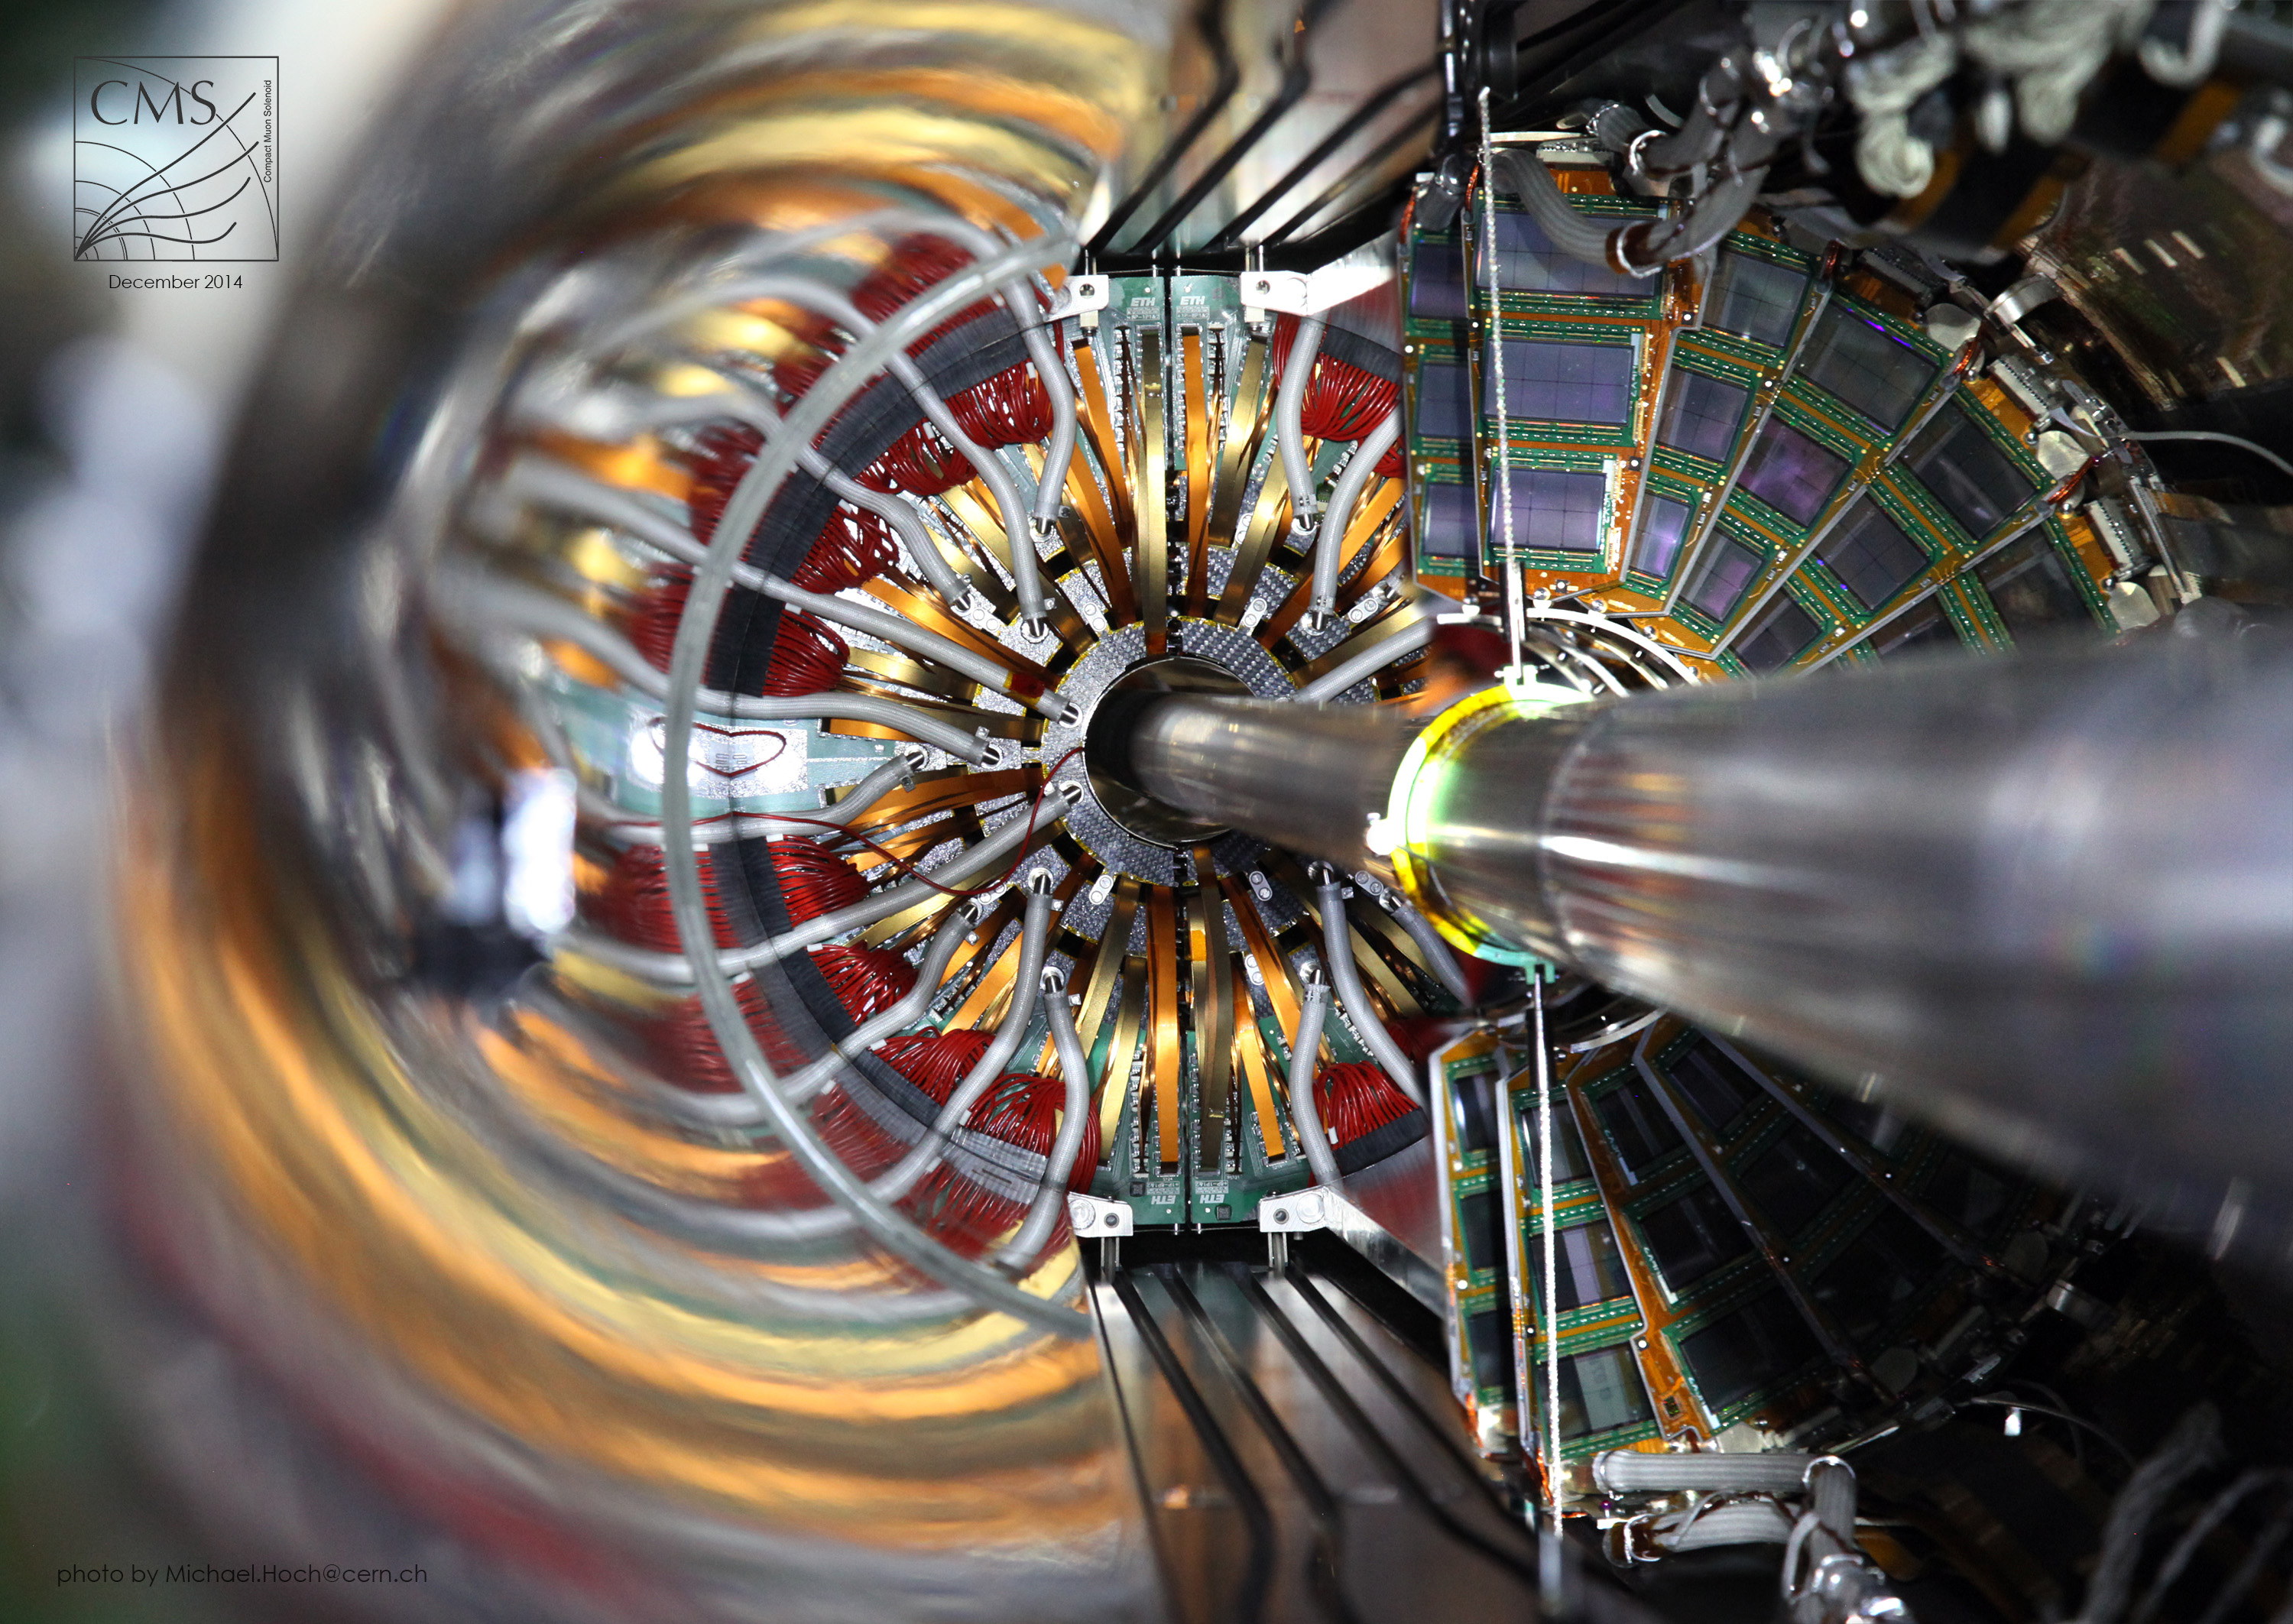
\includegraphics[width=0.88\textwidth]{figs/cms/a194Ts.jpg}
\vspace*{1mm}\caption{The pixel detector endcap disks being reinstalled around the beam pipe in December 2014 following Long Shutdown 1~\cite{Hoch:1977415}.}
\label{fig:pixel}
\end{center}
\end{figure}

The original detector was designed to operate under a nominal instantaneous luminosity of $1 \times 10^{34}\percms$.
With the LHC planning to deliver higher instantaneous luminosities with the same 25\ns bunch spacing following LS1, if no action was taken, the radiation damage from the increased \PU environment would result in the pixel tracker experiencing an unacceptable degradation in track reconstruction efficiency.
As such, it has been long recognised that the original pixel detector would require replacing at least once during LHC operations~\cite{CMS:1997tlf}.
Consequently, the original pixel tracker was completely replaced during the End of Year Technical Stop that took place between data taking in 2016 and 2017.
A detailed description of the Phase-I Pixel detector is given in~\cite{CMS:2012sda} as none of the results presented in this thesis involve data collected by the CMS experiment after 2016.
%%Like the original pixel detector, the Phase-I detector's 124 million pixels also measure $100 \times 150\mum^{2}$ (covering a total surface area of 1.95 $m^{2}$) and the sensors are also n+-type implants on n-type silicon.
%%The Phase-I Pixel detector is comprised of four 54.9\cm long barrel layers at mean radii of 3.0, 6.8, 10.9 and 16.0\cm and three endcap disks at each end of the barrel at $|z| = 29.1, 39.6 and 51.6\cm$ that extend from $r = 4.5 to 16.1\cm$.

\subsubsection{Silicon Microstrip Tracker}
As illustrated in Figure~\ref{fig:tracker}, the silicon microstrip detector is comprised of four parts: the Tracker Inner Barrel (TIB), Tracker Inner Disks (TID), Tracker Outer Barrel (TOB) and Tracker EndCaps (TEC).
The sensors are rectangular in the barrel region and trapezoid in the endcaps and all consist of single-sided strips of p$^{+}$-type implants on n-type silicon, which are connected to ROCs by aluminium strips.
A total of 9.3 million sensors are used across all four parts, covering a total area of 198 $\unit{m}^{2}$.

% CMS inner tracker barrel picture 
\begin{figure}[htbp]
\begin{center}
\vspace*{3mm}\includegraphics[width=0.92\textwidth]{figs/cms/0610026_01-3000.jpg}
\vspace*{2mm}\caption{The first half of the Tracker Inner Barrel (TIB) containing three layers of silicon strip modules~\cite{Maximilien:995912}.}
\label{fig:TIB}
\end{center}
\end{figure}

The TIB, shown in Figure~\ref{fig:TIB}, provides coverage in the range $20\cm < r < 55\cm$ and up to $|z| = 65\cm$ and is comprised of four layers.
The strips have a pitch of 80\mum for the inner two layers and 120\mum for the outer two layers, and a thickness of 320\mum and a typical length of 10\cm in each of the four layers.
The three disks on each side of the TIB form the TID, extends the inner microstrip tracker's coverage from $|z| = 65\cm$ to $|z| = 120\cm$.
Each disk is formed of three rings and the sensor pitches across the rings vary between 81-158\mum, but have a thickness of 320\mum throughout.

The TOB surrounds the TIB and TID and is comprised of six layers that provide coverage up to $|z| = 110\cm$.
In the outer microstrip tracker, increased strip thickness, length and pitch are used where the radiation levels are lower so that a similar occupancy and signal-to-noise ratio to that in the inner microstrip tracker can be maintained.
The pitch of the strips vary from 183\mum for the inner four layers to 122\mum for the outer two layers, with all having a thickness of 500\mum and a typical length of 25\cm. 
The TEC's nine disks per endcap extend coverage from $|z| = 120\cm$ to $|z| = 280\cm$, with the number of rings per disk varying from four to seven, depending on the disk's position in $z$.
The thickness of the sensors in the TEC are 320\mum in the three innermost rings and 500\mum in the rest respectively.

A number of ``stereo'' modules consisting of two back-to-back sensors are used in the inner two layers of the TIB and TOB, the inner two rings of the TID and rings one, two and five of the TEC.
These sensors are aligned at an angle of 100 mrad to each other, allowing measurements of both the $r-\phi$ and \rz coordinates, to a resolution of 23-34\mum in $r-\phi$ and 23\mum in z and 35–52\mum in $r-\phi$ and 52\mum in z in the TIB and TOB, respectively.

\subsection{Electromagnetic Calorimeter}\label{subsec:ECAL}
Beyond the tracker, the ECAL~\cite{CMS:1997ysd,CMS:2002xia}, a homogeneous calorimeter, measures the energies of electrons and photons using lead tungstate (PbWO$_{4}$) scintillating crystals.
The choice of detector technology was motivated by the need for the ECAL to be sufficiently compact to fit inside the solenoid along with the HCAL, while containing the EM showers' energy within the ECAL.
Therefore, lead tungstate crystals were chosen due to their short radiation length (0.89\cm) and small Molier\'{e} radius (2.2\cm).
The crystals also have a high radiation tolerance and have a short scintillation delay time, with 80\% of the scintillated light being emitted within one 25\ns bunch crossing.

The ECAL barrel and each of the ECAL endcaps contain 61,200 and 7,324 crystals, respectively, with each crystal having a granularity of 0.0174 in the $\eta - \phi$ plane.
As the PbWO$_{4}$) crystals emit a relatively low light yield, photodetectors are required to amplify this light.
Avalanche photodiodes are used in the barrel and the more radiation hard vacuum phototriodes in the endcap disks, respectively, to amplify the light and convert it into an electrical current that is directly proportional to the energy of the induced electromagnetic showers.
These signals are digitised on-detector and buffered until a Level-1 Trigger decision has been made.

The layout of the ECAL system is displayed in Figure~\ref{fig:ecal}, illustrating the layout of both the barrel (EB) and endcap (EE) cystal systems, the gap between the EB and EE, and the Preshower (ES)~\cite{Loos:539819} device located in front of the ECAL endcaps.

\begin{figure}[htb]
\begin{center}
\vspace*{4mm}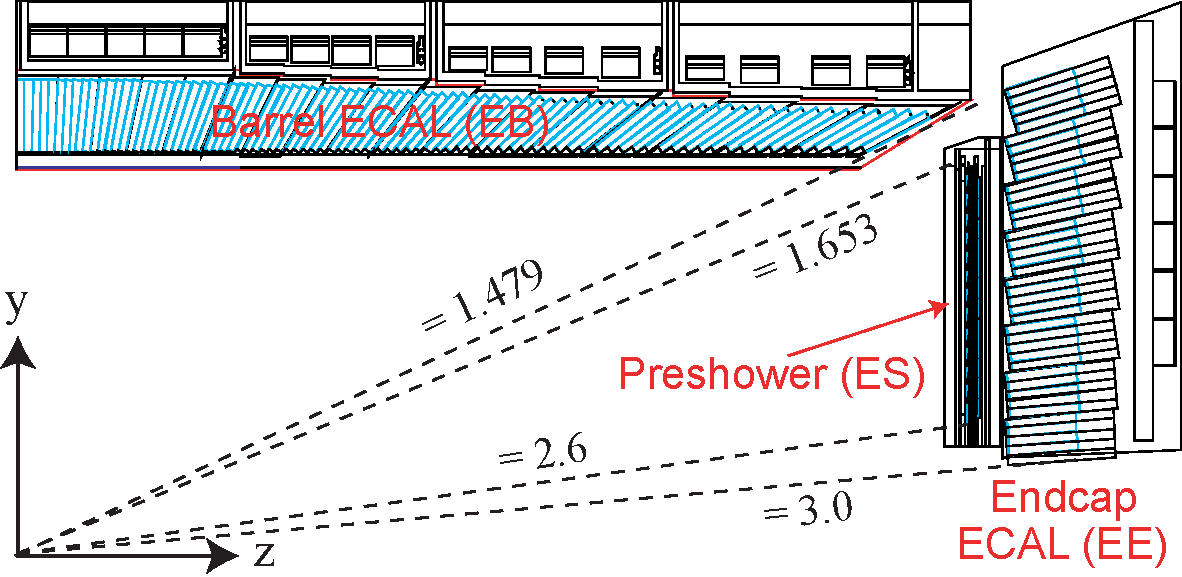
\includegraphics[width=0.9\textwidth]{figs/cms/ECAL_Transverse_section.pdf}
\caption{Layout of one quadrant of the ECAL system, illustrating the locations of the barrel ECAL (EB), endcap ECAL (EE) and ECAL Preshower (ES) device~\cite{Bayatian:2006nff}.}
\label{fig:ecal}
\end{center}
\end{figure}

The ES aids the EE system in discriminating between neutral pions and photons within the fidicial region $1.653 < |\eta| < 2.6$.
For each ES, two lead radiators initiate the electromagnetic showers and two silicon strip sensors, orthogonal to one another to provide fine resolution, are placed after the radiators.
The thickness of the radiators was chosen to be two and one radiation lengths for the first and second lead radiators, respectively, in order to ensure that ~95\% of incident photons shower before reaching the second silicon strip sensor.

ECAL test beam measurements~\cite{Adzic:2007mi} of the PbWO$_{4}$ crystals in the absence of a magnetic field have determined the energy resolution, $\sigma_{E}$, to be,

\begin{equation}
(\frac{\sigma_{E}}{E})^{2} = (\frac{2.8\%}{\sqrt{E}})^{2} + (\frac{12\%}{E})^{2} + (0.3\%)^{2} \;.
\label{eq:ecalResolution}
\end{equation}

where E is the energy of the incident electron in \GeV. 
The first term is the stochastic term representing the statistical fluctuations in the amount of photo-electrons produced, the second term is the nosie term which represents the noise from the electronics and digitisation, and the third term is the constant term which covers any non-uniform longitudinal response and shower containment losses~\cite{Adzic:2007mi}.

% Relative electron energy resolution unfolded in bins of pseudo rapidity for the barrel and the endcaps using electrons from Z → ee decays. The resolution is shown for low (left) and high (right) bremsstrahlung electrons (R9 > 0.94 and R9 < 0.94 respectively, with R9 = E3x3/ESupercluster).
% Relative energy resolution for electrons with minimal effect of bremsstrahlung:𝐸3×3∕𝐸supercluster≥0.94.
%Sun:2016fvz

\subsection{Hadronic Calorimeter}\label{subsec:HCAL}
Hadronic particles pass through the ECAL and enter the HCAL~\cite{HCAL:tdr}.
The HCAL measures the energies of the resulting hadronic jets and contains them for the accurate determination of the missing transverse energy~\cite{HCAL:tdr}.
As such, the HCAL was designed to have as much absorber material within the solenoid coil as practical. 

The barrel (HB) and endcaps (HE) both use plastic scintillator tiles which are interspersed between brass and steel absorber plates.
Steel is used for the innermost and outermost HB and HE absorber plates for structural strengthening.
The HB covers the rapidity range $|\eta| < 1.4$, with the HE providing coverage over the range $1.3 < |\eta| < 3.0$.
Both the HB and HE are segmented in $\eta - \phi$ by $0.087 \times 0.087$ for $| \eta | < 1.6$ and up to $0.17 \times 0.17$ for $| \eta | >= 1.6$.
Wavelength shifting fibres embedded in the tiles are used convert the scintillation light and channel it to hybrid photodiodes.

The forward hadronic calorimeters (HF) extends coverage up to $\eta < 5.2$ region~\cite{HF}.
As the very forward region experiences the highest radiation dose, quartz fibres, interspaced between steel absorbers, are used instead due to their radiation hardness and fast response time.
The quartz fibres produce Cherenkov radiation above a certain energy threshold (thus ignoring low energy particles) and are able to give directional information due to the light being strongly correlated with the showers' trajectories.
The Cherenkov light is transmitted down the fibres to individually shielded photomultiplier tubes contained in readout boxes.

Due to space constraints within the solenoid, the 5.8 to 10.6 interactions lengths of absorber material within the HB is insufficient to fully contain highly penetrating jets.
Therefore, the HB is supplemented by an additional calorimeter in the barrel region outside the coil known as the HO~\cite{HO}.
With the solenoid's coil, which acts as an additional absorber, the HO increases the effective absorber thickness to at least 11.8 interaction lengths.

Using test beam measurements using electrons, muons and pions, the combined energy resolution of the ECAL and HCAL together, in terms of the stochastic and constant terms, was determined to be

\begin{equation}
(\frac{\sigma_{E}}{E})^{2} = (\frac{84.4 \pm 1.6\%}{\sqrt{E}})^{2} + (7.4 \pm 0.8\%)^{2} \;.
\label{eq:hcalResolution}
\end{equation}

for the HB and HE~\cite{Abdullin:2008zzb}, and

\begin{equation}
(\frac{\sigma_{E}}{E})^{2} = (\frac{198\%}{\sqrt{E}})^{2} + (9\%)^{2} \;.
\label{eq:hfResolution}
\end{equation}

for the HF~\cite{Bayatian:2006jz}.

\subsection{The Superconducting Solenoid}\label{subsec:magnet}
One of the defining features of the CMS detector is the superconducting solenoid, that encompasses the silicon tracker and calorimetry~\cite{Acquistapace:1997fm,Herve:2000}.
The cylindrical coil measures 13\,m long, has a 5.9\,m inner diameter, is situated inside a vacuum tank where it is cooled to its operating temperature of 4.5\,K using liquid helium, and operates at magnetic field of 3.8\,T.
While the solenoid was designed to operate at 4\,T, the CMS Collaboration chose to operate it at 3.8\,T in order maximise the lifetime of the apparatus.

As shown in Figure~\ref{fig:magneticField}, the solenoid provides a strong homogenous magnetic field within its volume.
This large bending power not only provides excellent momentum resolution for charged particles within the tracking detector, but it also prevents low transverse momentum charged particles from reaching the calorimetry and negatively impacting on energy resolution and isolation efficiency.
Outside the solenoid, an iron return yoke guides and contains the return magnetic field.
The return magnetic field is approximately 1.7\,T in the barrel and outermost endcap disks which is sufficiently strong to enable accurate momentum resolution for tracking and charge identification of high momentum, \ie $\geq 1\TeV$, muons.

\begin{figure}[htb]
\begin{center}
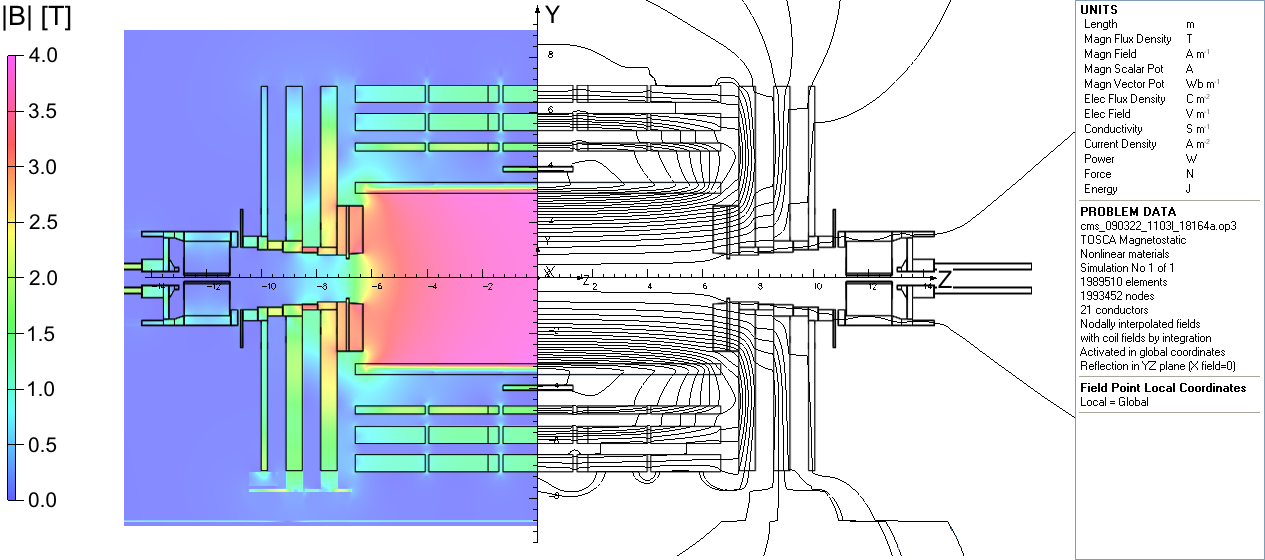
\includegraphics[width=0.97\textwidth]{figs/cms/cms_magnetic_field.png}
\caption{Longitudinal section of the CMS detector, illustrating the predicted magnetic field strength (left) and field lines (right) for the operational central magnetic flux density of 3.8\,T~\cite{Chatrchyan:2009si}.}
\label{fig:magneticField}
\end{center}
\end{figure}

\subsection{Muon Detectors}\label{subsec:muon chambers}
As implied by the experiment's name, the detection and measurement of muons is incredibly important for CMS, as many of the signatures of interesting events involve them.
As muons are Minimum Ionising Particles (MIPs), they pass through the inner detectors and the solenoid with minimal interaction.
Consequently, the muon chambers~\cite{CMS:1997iti} are placed outside the solenoid and are interspaced between the iron return yoke rings and disks.

Figure~\ref{fig:muonChambers} shows the layout of the gas detectors which make up the muon system.
As the magnetic field outside the solenoid is non-uniform and the radiation levels vary, the muon system is comprised of three different types of detectors that use different technologies in order to provide a high performance system. 

\begin{figure}[htbp]
\begin{center}
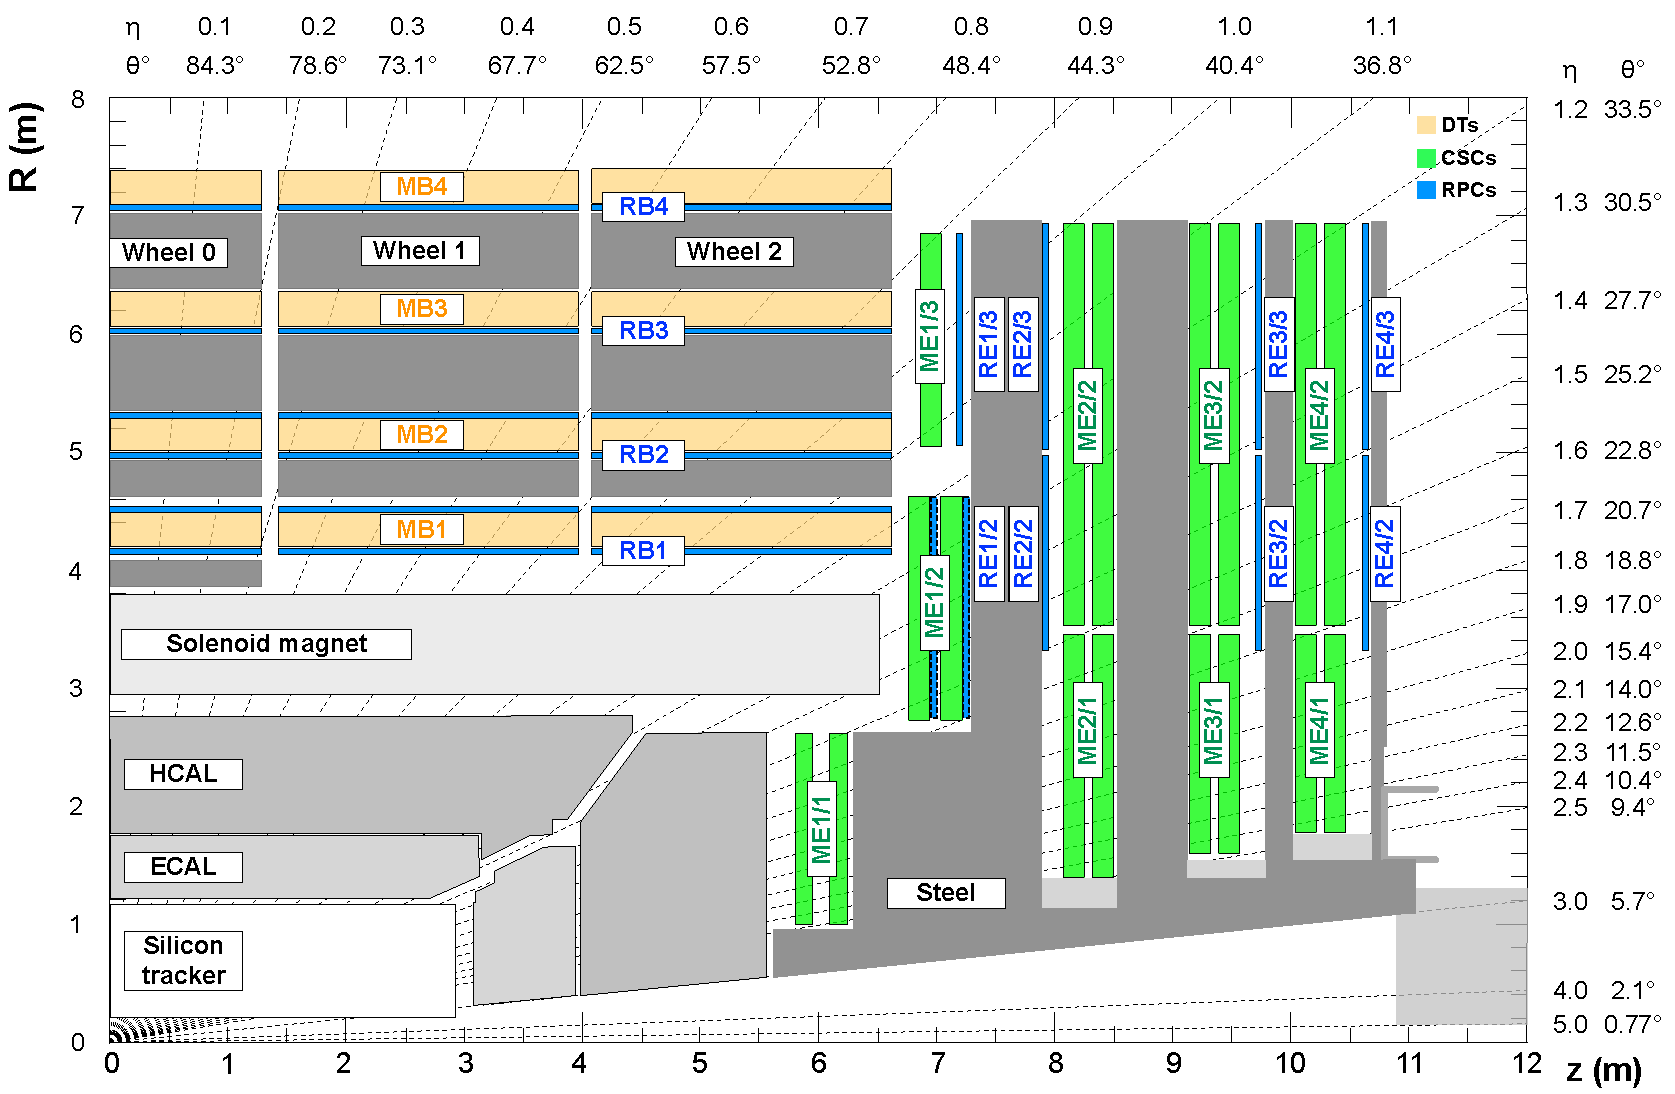
\includegraphics[width=0.97\textwidth]{figs/cms/cms_muon_quadrant_run_ii.pdf}
\caption{Layout of one quadrant in \r-z of the CMS muon detectors in their current configuration.
The DTs are marked in yellow, the CSCs in green and the RPCs in blue~\cite{CMS-DP-2016-046}.}
\label{fig:muonChambers}
\end{center}
\end{figure}

Drift Tubes (DTs) operate in the barrel region covering $|\eta| < 1.2$, where the magnetic field strength is low as most of the return field is contained within the return yoke.
Each tube is a $4.2\cm \times 1.3\cm$ cell that contains an anode wire surrounded by a mixture of Ar (85\%) and CO$_{2}$ (15\%).
As a muon passes through the chamber it ionises the gas within, with the resultant free electrons drifting towards the positively charged wire and inducing an electrical signal that is read out.

\begin{figure}[htb]
\begin{center}
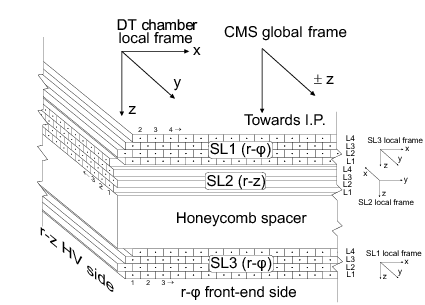
\includegraphics[width=0.8\textwidth]{figs/cms/DTchamber.png}
\caption{A schemeatic layout of a DT chamber, illustrating the half DT width offset between the adjacent layers and the $r-\phi$ plane orientation of the outer SLs and the \rz plane orientation of the inner layer~\cite{Chatrchyan:2009hg}.}
\label{fig:dtSuperLayers}
\end{center}
\end{figure}

As shown in Figure~\ref{fig:dtSuperLayers}, the DT chambers are comprised of twelve layers of DTs that are grouped into three \emph{superlayers} (SLs) of DTs.
Each SL is comprised of four layers of DTs, with each layer being offset from the other by half the width of half a DT in order to improve angular resolution.
The outer SLs are orientated to measure coordinates in the $r-\phi$ plane and the innermost SL is orientated to measure coordinates in the \rz plane (which the outermost station lacks).
A honeycomb spacing structure separates SL3 from the other SLs to increase the lever arm length for measuring the track direction in the bending plane.
This arrangement allows for a high muon track identification efficiency and provides resolutions of about $200\mum$ and a $\phi$ angular resolution of approximately $1$ mrad.

Cathode Strip Chambers (CSCs) are employed across four endcap disks which cover the region $0.9 < \eta < 2.4$.
SCS are used in the endcaps as they are more suited to the higher muon rate and non-uniform magnetic field environment of the forward regions.
While only the innermost ring of the outermost (fourth) disk was originally installed, an outer ring for the outermost disk was installed during LS1 during 2013-2015~\cite{Battilana:2017mrm}.

\begin{figure}[htb]
\begin{center}
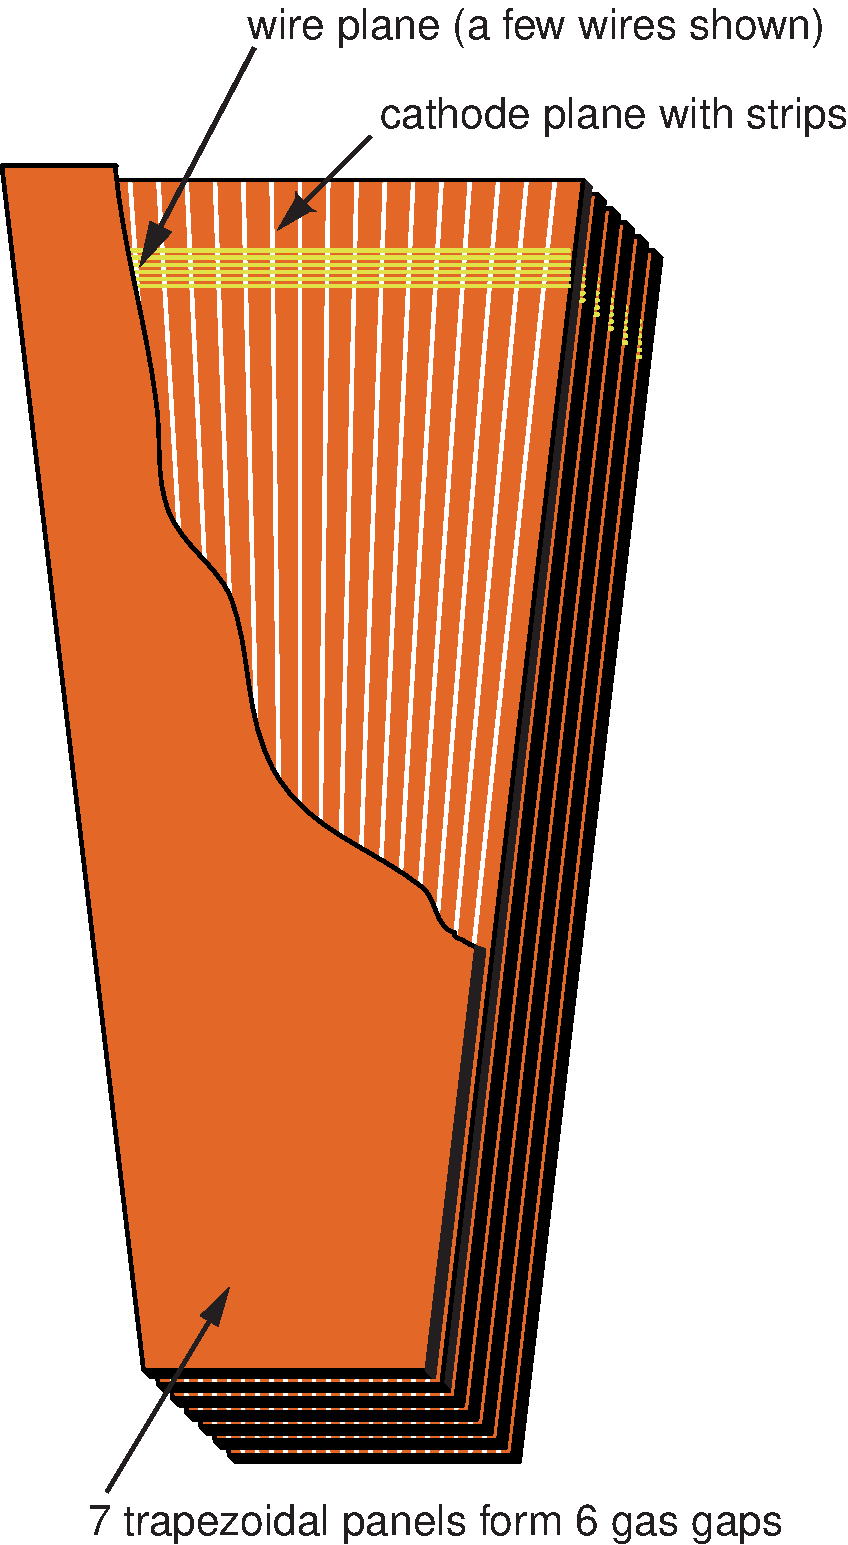
\includegraphics[width=0.45\textwidth]{figs/cms/csc_trapezoid_v1.pdf}
\caption{A schemeatic overview of a CSC, illustrating a plane of anode wires between two of the trapezoidal panels and the plane of cathode strips which run almost perpendicular to them~\cite{Bayatian:2006nff}.}
\label{fig:csc}
\end{center}
\end{figure}

Each CSC, as shown in Figure~\ref{fig:csc}, is composed of seven trapezoidal panels. 
The six gaps between the panels are filled with planes of anode wires that run almost perpendicular to a planes of cathode strips which are surrounded by a gas mixture of Ar, CO$_{2}$ and CF$_{4}$~\cite{Anderson:2004ep}.
This provides six position measurements per chamber with a resolution in the $r-\phi$ plane of 75\mum for the two innermost rings of the first disk and 150\mum for the other disks~\cite{CMS:1997iti}.

Resistive Plate Chambers (RPCs) provide complimentary coverage in the range $|\eta| < 1.8$~\cite{Battilana:2017mrm}.
The barrel contains six layers of RPCs, with a layer either side of the first two DT layers and one in each of the outer stations, and the endcaps have 4 RPC disks each, one for each CSC disk.

Each RPC is formed of two parallel resistive plates, separated by a gas filled gap of a few millimetres, with a large electric field applied across it.
In contrast to the DTs and CSCs, RPCs have a coarser position resolution of about 1\cm but have faster response times and a superior excellent time resolution of approximately $2\ns$.
Consequently, the RPCs are used by trigger system to identify muons and to accurately determine which bunch crossing they originated from.
Their coarser spatial resolution is also used to supplement information from the DTs and CSCs in track reconstruction.

When the information from the muon and tracker systems are combined, as described in Chapter~\ref{chapter:data-mc}, the CMS detector is able to measure momentum resolutions of $1.3\%$ to $2.0\%$ in the barrel and up to $6\%$ in the endcaps and a charge misidentification rate of less than $0.1\%$ for muons with \pT less than $100 \GeV$~\cite{Chatrchyan:2012xi,Chatrchyan:2013sba}.

\subsection{Trigger and Data Acquisition Systems}\label{subsec:trigger}
At design luminosity, the LHC has a bunch crossing (BX) rate of $40\MHz$, i.e. of the order of $10^{9}$ inelastic events per second.
With each proton-proton collision event having a size of about $1.5$MB~\cite{Bayatian:2006nff}, even if there was processing power and sufficient bandwidth available to reconstruct the read-out of all the sub-detectors for every event, there would be insufficient storage capacity to save them.

The vast majority of events however, are uninteresting from a physics perspective, with the cross sections of interesting processes being at least a factor of $10^{7}$ smaller than the total proton-proton cross section of $110.6 \pm 3.4$ mb~\cite{Antchev:2017dia}.
Consequently, the CMS trigger system is designed to reject these background events and select events in a manner that allows all possible new physics signatures to be detected whilst keeping acceptance thresholds sufficiently as low as reasonably possible.

The CMS trigger system is comprised of two stages, the Level-1 (L-1) Trigger and the High Level Trigger (HLT), as it is not feasible to reduce the data rate in a single processing stage without compromising on physics performance.
Since initial operations of the CMS experiment, the original event storage rate of 100\Hz has been increased to 0.5-1\kHz~\cite{Dasu:2000ge,phase1L1TDR}.

\subsubsection{Level-1 Trigger}\label{paragraph:L1}
The Level-1 trigger reduces the input $40\MHz$ rate to about $100\kHz$ and consists of FPGAs (Field Programmable Gate Arrays) and ASICs (Application Specific Integrated Circuits), which have to be highly efficiency at identifying interesting physics signals.
As the trigger decision cannot be made before the subsequent BX, the L-1 Trigger uses a pipelined approach that is capable of buffering the detector for about 3.8\mus (limited by the tracker and ES buffers) before a decision has to be made on whether to read-out an event or discard it. 
This latency precludes both the reading out of events in full and of the use of iterative reconstruction algorithms.
While the calorimeters and muon detectors contribute to the L-1 Trigger decision, tracking information does not as as when CMS was designed it was not possible to read out every event from the tracker.

The current L-1 trigger, the \emph{Phase-I Trigger}, was developed to ensure that the 100\kHz L1 trigger limit would be maintained following the increase in the instantaneous luminosity and centre-of-mass energy of the LHC following LS1~\cite{phase1L1TDR}.
The Phase-I Calorimeter Trigger is based on a \emph{time-multiplexed} architecture which uses large FPGAs on a small number of general-purpose boards with fast optical links that allow for full granularity data to be used.
The previous calorimeter trigger architecture reduced the volume of input data by identifying the best trigger candidates at a regional level and forwarding them to a global stage where a L-1 acceptance decision would be made~\cite{phase1L1TDR}.
In contrast, time-multiplexed trigger concept processes full granularity data from across the calorimetry systems for every \emph{n}th bunch crossing on one of \emph{n} identical processors.
Such a system requires at least two layers, linked by a switching network which buffers and transmits data from the multiple sources to a single processor, as illustrated in Figure~\ref{fig:TMT}.

\begin{figure}[htbp]
\begin{center}
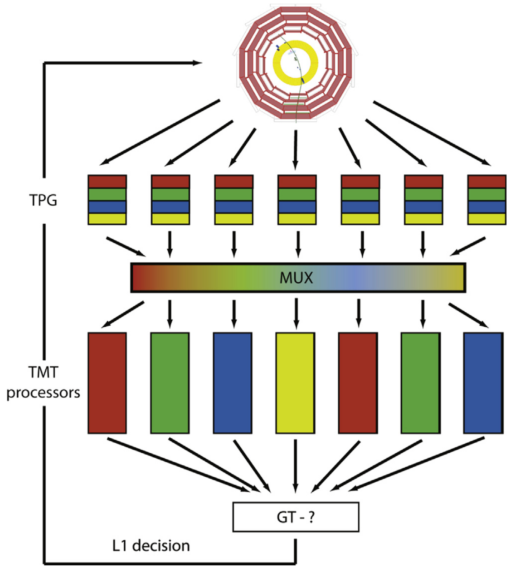
\includegraphics[width=0.97\textwidth]{figs/cms/TMT.pdf}
\caption{In a time-multiplexed trigger, all data from the Trigger Primitive Generators (TPG) covering the entire detector are transmitted to one of ``n'' identical processors after passing through the multiplexing fabric (MUX), a serial interconnection linking each TPG to each TMT processor, before being passed to the Global Trigger (GT) where the decision of whether or not to issue a L1 receipt to the HLT is determined~\cite{tmttelba}.}
\label{fig:TMT}
\end{center}
\end{figure}

A time-multiplexed architecture was used as it provided a number of advantages compared to traditional trigger architectures, including:
\begin{itemize}
\item minimised boundary issues and data sharing between processors, saving time and resources and allowing for data from the entire calorimeter for a bunch crossing to be considered on a single processor and thus consider candidates that would have been discarded by the previous regional triggers;
\item synchronisation being only required within each processor instead of the entire system;
\item system demonstration with a single processor as each processor is identical and fully pipelined (no sideways connections);
\item validation only requiring one processor as each is identical and has no sideways communication;
\item the loss of a processor resulting in the loss of a bunch crossing instead of a region of the detector;
\item the use of spare processors to test new algorithms online in parallel with the nominal trigger without affecting the current system and as backup processors in case of the failure of another.
\end{itemize} 

The electronics of the Phase-I Trigger were installed during LS1 and ran using the legacy trigger system during 2015 with the new trigger system running in parallel for validation prior to commissioning and usage during 2016~\cite{Zabi:2017lya}.

Given the operational successes of this architecture, a similar time-multiplexed approach for a proposed track finding system for the Phase-II Outer Tracker has been developed.
This proposed system and the studies presented in this thesis relating to it are discussed in Chapter~\ref{chapter:tk-upgrade}.

\subsubsection{High Level Trigger and Data Acquisiation}\label{paragraph:HLT}
Upon receipt of a L1 trigger, the Data Acquisition (DAQ) system reads out the buffered data from the detector front-end electronics and collates it into a complete event to be processed by the HLT~\cite{Sphicas:2002gg}.

The HLT is a high performance computing farm comprised of commercially available processors running the CMS Software (known as \CMSSW) which reduces the L1 rate of about $100\kHz$ to an output rate of approximately $1\kHz$.
In contrast to the L1 trigger, the HLT has a larger latency budget and is able to make use of the full detector readout (including the Tracker and ES), allowing for more sophisticated reconstruction and selection algorithms to be used to select events for storage.
This however, does not mean that the full event is reconstructed, as such a task is too CPU intensive to be done online within the latency constraints.
Events accepted by the HLT are forwarded to the offline Tier-0 computing centre for offline processing and reconstruction and are also passed to the online detector monitoring systems.

\subsection{LHC and CMS Performance}\label{subsec:Lumi}
During 2016, the LHC operated at $\sqrt{s} = 13\TeV$ up to a maximum instantaneous luminosity of $15.3 \times 10^{33}$ \percms.
As shown in Figure~\ref{fig:cms_lumi}, the LHC delivered a total integrated luminosity of 40.82\fbinv during stable beams to the CMS detector, of which 37.76\fbinv was recorded~\cite{cmsLumiPage,CMS:2017_lumi}.
\begin{figure}[htbp]
\begin{center}
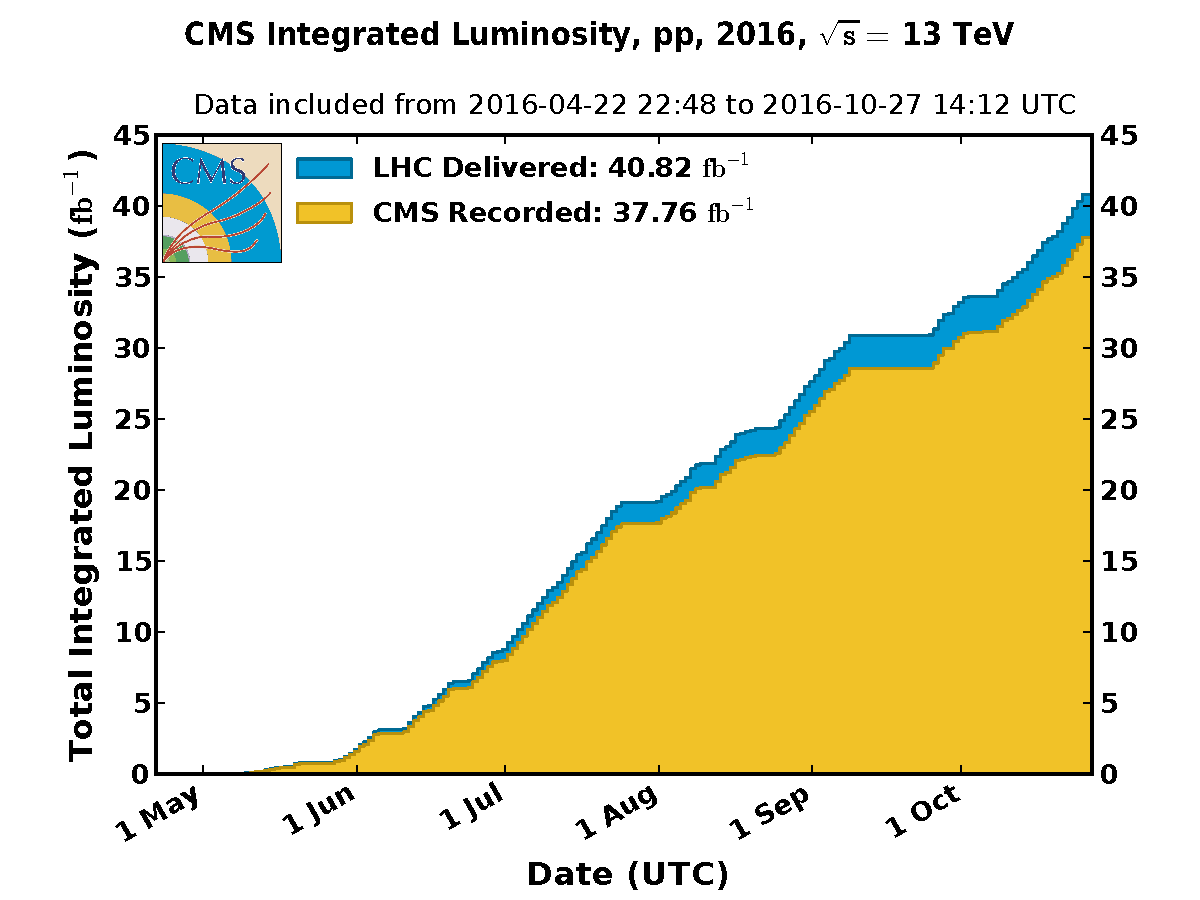
\includegraphics[width=1.05\textwidth]{figs/lhc/int_lumi_per_day_cumulative_pp_2016.pdf}
\caption{The total integrated luminosity delievered to and recorded by the CMS experiment during 2016~\cite{CMS:2017_lumi}.}
\label{fig:cms_lumi}
\end{center}
\end{figure}

The CMS experiment monitors and measures the instantaneous and integrated luminosity delivered by the LHC using the pixel detector, DTs, HF, the Fast Beam Conditions Monitor and Pixel Luminosity Telescope.
During Run 2 of the LHC, the primary offline luminosity measurements made by the CMS Luminosity Group used the pixel detector using the Pixel Cluster Counting (PCC) method due its stability over time for up an average \PU of 150 and the high precision results obtained with it during Run 1.
The PCC algorithm is able to achieve such a precision by measuring the instantaneous luminosity through the number of pixels present. 
This is possible as the probability of pixel hit belonging to multiple tracks is very small due to the very low occupancy of the detector, inferring that the number of pixel hits are linearly proportional to the number of interactions during a bunch crossing~\cite{CMS:2017_lumi}.

Van der Meer (VdM) scans during dedicated LHC runs were used to calibrate the absolute luminosity scale calibrations of the detectors~\cite{vanderMeer:1968zz}
